\documentclass[11pt]{article}
\usepackage{cornell-notes}
\usepackage{mathtools}
\usepackage{needspace}
\usepackage{ragged2e}
\usepackage{adjustbox}
\usepackage{tikz}
\usetikzlibrary{arrows.meta,positioning}
\tcbuselibrary{most}
\geometry{letterpaper,margin=0.72in,headheight=15pt}
\setCornellCollection{Calculus Cornell Notes}
\setCornellUnitType{Chapter}
\setCornellUnitNumber{2}
\setCornellUnitTitle{Differentiation}

\definecolor{Ink}{HTML}{17324D}
\definecolor{Teal}{HTML}{147D78}
\definecolor{Sky}{HTML}{DDEEF1}
\definecolor{Cue}{HTML}{EEF2F5}
\definecolor{Warm}{HTML}{FFF3D6}
\definecolor{Alert}{HTML}{9D3C32}
\definecolor{Green}{HTML}{276749}
\definecolor{Rule}{HTML}{AAB8C2}
\hypersetup{colorlinks=true,linkcolor=Ink,urlcolor=Teal,pdfborder={0 0 0}}
\setlength{\parindent}{0pt}
\setlength{\parskip}{4pt}
\setlist{nosep,leftmargin=*}
\titleformat{\section}{\Large\bfseries\color{Ink}}{}{0pt}{}[\color{Teal}\titlerule]
\titleformat{\subsection}{\large\bfseries\color{Teal}}{}{0pt}{}
\pagestyle{fancy}
\fancyhf{}
\fancyhead[L]{\small\color{Ink}\textsc{Cornell Notes}}
\fancyhead[R]{\small\color{Teal}\nouppercase{\leftmark}}
\fancyfoot[L]{\footnotesize\color{Ink}Active recall $\bullet$ Worked reasoning $\bullet$ Verification}
\fancyfoot[R]{\footnotesize\color{Ink}\thepage\ of \pageref*{LastPage}}
\renewcommand{\headrulewidth}{0.5pt}
\renewcommand{\footrulewidth}{0.4pt}
\newcolumntype{Y}{>{\RaggedRight\arraybackslash}X}
\newtcolorbox{orientationbox}{enhanced,breakable,colback=Sky,colframe=Teal,boxrule=0.7pt,arc=2mm,title=Chapter orientation,fonttitle=\bfseries}
\newtcolorbox{sectionsummarybox}{enhanced,breakable,colback=white,colframe=Teal,boxrule=0.6pt,arc=1.5mm,left=2mm,right=2mm,top=1mm,bottom=1mm,title=Section synthesis,fonttitle=\bfseries\color{Teal}}
\newtcolorbox{warningbox}{enhanced,breakable,colback=Warm,colframe=Alert,boxrule=0.7pt,arc=1.5mm,title=Common error audit,fonttitle=\bfseries}
\newtcolorbox{checkbox}{enhanced,breakable,colback=white,colframe=Green,boxrule=0.7pt,arc=1.5mm,title=Verification habit,fonttitle=\bfseries}
\newcommand{\cornellcuehead}{\rowcolor{Ink}\color{white}\bfseries Cue / recall prompt & \color{white}\bfseries Notes / reasoning \\\endhead}
\newcommand{\cornellcuerow}[2]{\rowcolor{Cue}#1 & #2 \\\addlinespace[3pt]}
% Table-safe: delegates to the shared Cornell formula box (cornell-notes.sty),
% which cannot emit \pagebreak/\noalign inside longtable cells.
\newcommand{\formula}[1]{\CornellFormula[colback=Sky,colframe=Teal]{#1}}

\title{Chapter 2: Differentiation\\[2mm]\large Cornell Notes}
\author{}
\date{}
\hypersetup{pdftitle={Chapter 2: Differentiation - Cornell Notes},pdfauthor={},pdfsubject={Calculus study notes},pdfkeywords={calculus, Cornell notes, active recall}}
\begin{document}
\maketitle
\thispagestyle{fancy}
\begin{orientationbox}
Turn the limit definition of instantaneous change into a practical differentiation toolkit for explicit, composite, implicit, and time-dependent relations. These notes follow the complete local section sequence (99--164) and emphasize definitions, governing results, strategy selection, and verifiable reasoning.
\end{orientationbox}

\section{Prerequisite map}
\begin{minipage}[t]{0.42\textwidth}
\textbf{Bring forward}
\begin{itemize}
\item Limits
\item Function algebra
\item Trigonometric functions
\item Equations of lines
\end{itemize}
\end{minipage}\hfill
\begin{minipage}[t]{0.54\textwidth}
\textbf{Chapter flow}
\begin{center}
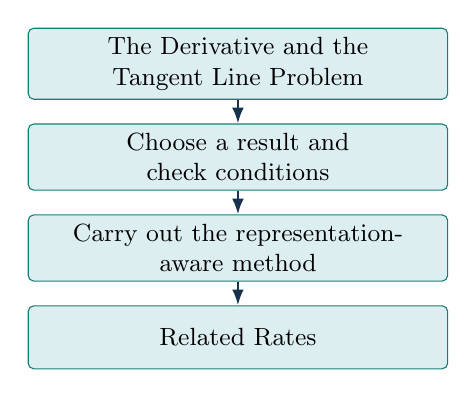
\begin{tikzpicture}[node distance=3mm, every node/.style={font=\small,align=center}, box/.style={draw=Teal,rounded corners=2pt,fill=Sky,minimum height=8mm,text width=0.42\textwidth}, arr/.style={-{Latex[length=2mm]},thick,draw=Ink}]
\node[box] (a) {The Derivative and the Tangent Line Problem};
\node[box,below=of a] (b) {Choose a result and check conditions};
\node[box,below=of b] (c) {Carry out the representation-aware method};
\node[box,below=of c] (d) {Related Rates};
\draw[arr] (a)--(b); \draw[arr] (b)--(c); \draw[arr] (c)--(d);
\end{tikzpicture}
\end{center}
\end{minipage}

\section{Learning objectives}
\begin{enumerate}
\item Explain the central objects and hypotheses in 2.1 and 2.6.
\item Translate among algebraic, graphical, numerical, and verbal representations.
\item Select an appropriate formula or theorem before beginning symbolic work.
\item Carry out multi-step calculations while preserving domain, sign, orientation, and units.
\item Diagnose common errors by testing assumptions and checking the result independently.
\item Synthesize the chapter's methods into a reusable problem-solving workflow.
\end{enumerate}

\section{2.1 The Derivative and the Tangent Line Problem}
\begin{longtable}{C N}\cornellcuehead
\cornellcuerow{What is the governing idea in 2.1?}{The derivative is the limiting slope of secant lines and gives the best local linear rate of change.}
\cornellcuerow{Which result should be recalled?}{\formula{f'(a)=\lim_{h\to0}\frac{f(a+h)-f(a)}{h}}}
\cornellcuerow{How should a problem be organized?}{Form the difference quotient, simplify before taking the limit, and use point-slope form for the tangent line.}
\cornellcuerow{What should be checked before accepting an answer?}{Confirm the hypotheses and domain, preserve units and orientation when relevant, and substitute or differentiate back into the defining relation.}
\end{longtable}
\begin{warningbox}Substituting $h=0$ before simplifying produces the indeterminate form that the limit is designed to resolve.\end{warningbox}
\begin{sectionsummarybox}The derivative is the limiting slope of secant lines and gives the best local linear rate of change. The operational habit is to form the difference quotient, simplify before taking the limit, and use point-slope form for the tangent line.\end{sectionsummarybox}
\section{2.2 Basic Differentiation Rules and Rates of Change}
\begin{longtable}{C N}\cornellcuehead
\cornellcuerow{What is the governing idea in 2.2?}{Power, constant, and sum rules make derivatives efficient, while units determine the interpretation of a rate.}
\cornellcuerow{Which result should be recalled?}{\formula{\frac{d}{dx}x^n=nx^{n-1}}}
\cornellcuerow{How should a problem be organized?}{Rewrite radicals and reciprocals as powers, differentiate term by term, and attach output-units per input-unit to the result.}
\cornellcuerow{What should be checked before accepting an answer?}{Confirm the hypotheses and domain, preserve units and orientation when relevant, and substitute or differentiate back into the defining relation.}
\end{longtable}
\begin{warningbox}The derivative of a constant is zero; reducing the exponent without multiplying by the old exponent is a common error.\end{warningbox}
\begin{sectionsummarybox}Power, constant, and sum rules make derivatives efficient, while units determine the interpretation of a rate. The operational habit is to rewrite radicals and reciprocals as powers, differentiate term by term, and attach output-units per input-unit to the result.\end{sectionsummarybox}
\section{2.3 Product and Quotient Rules and Higher-Order Derivatives}
\begin{longtable}{C N}\cornellcuehead
\cornellcuerow{What is the governing idea in 2.3?}{Products and quotients require interaction rules; repeated differentiation measures changing rates such as acceleration.}
\cornellcuerow{Which result should be recalled?}{\formula{(fg)'=f'g+fg',\qquad \left(\frac fg\right)'=\frac{f'g-fg'}{g^2}}}
\cornellcuerow{How should a problem be organized?}{Label component functions, apply the correct rule without premature expansion, simplify afterward, and preserve denominator restrictions.}
\cornellcuerow{What should be checked before accepting an answer?}{Confirm the hypotheses and domain, preserve units and orientation when relevant, and substitute or differentiate back into the defining relation.}
\end{longtable}
\begin{warningbox}Differentiating a product as $f'g'$ or reversing the quotient numerator changes the function.\end{warningbox}
\begin{sectionsummarybox}Products and quotients require interaction rules; repeated differentiation measures changing rates such as acceleration. The operational habit is to label component functions, apply the correct rule without premature expansion, simplify afterward, and preserve denominator restrictions.\end{sectionsummarybox}
\section{2.4 The Chain Rule}
\begin{longtable}{C N}\cornellcuehead
\cornellcuerow{What is the governing idea in 2.4?}{The derivative of a composition multiplies the outer rate by the inner rate.}
\cornellcuerow{Which result should be recalled?}{\formula{\frac{d}{dx}f(g(x))=f'(g(x))g'(x)}}
\cornellcuerow{How should a problem be organized?}{Identify layers from outside to inside, differentiate each active layer, and multiply the factors before simplifying.}
\cornellcuerow{What should be checked before accepting an answer?}{Confirm the hypotheses and domain, preserve units and orientation when relevant, and substitute or differentiate back into the defining relation.}
\end{longtable}
\begin{warningbox}Stopping after the outer derivative omits the inner scaling and usually gives a locally wrong rate.\end{warningbox}
\begin{sectionsummarybox}The derivative of a composition multiplies the outer rate by the inner rate. The operational habit is to identify layers from outside to inside, differentiate each active layer, and multiply the factors before simplifying.\end{sectionsummarybox}
\section{2.5 Implicit Differentiation}
\begin{longtable}{C N}\cornellcuehead
\cornellcuerow{What is the governing idea in 2.5?}{When $x$ and $y$ are linked by an equation, differentiate both sides with respect to $x$ and treat $y$ as $y(x)$.}
\cornellcuerow{Which result should be recalled?}{\formula{\frac{d}{dx}F(x,y)=F_x+F_y\frac{dy}{dx}=0}}
\cornellcuerow{How should a problem be organized?}{Differentiate every term, attach $y'$ whenever a $y$-expression is differentiated, collect $y'$ terms, then solve.}
\cornellcuerow{What should be checked before accepting an answer?}{Confirm the hypotheses and domain, preserve units and orientation when relevant, and substitute or differentiate back into the defining relation.}
\end{longtable}
\begin{warningbox}Forgetting the chain factor on terms such as $y^n$ is the characteristic implicit-differentiation mistake.\end{warningbox}
\begin{sectionsummarybox}When $x$ and $y$ are linked by an equation, differentiate both sides with respect to $x$ and treat $y$ as $y(x)$. The operational habit is to differentiate every term, attach $y'$ whenever a $y$-expression is differentiated, collect $y'$ terms, then solve.\end{sectionsummarybox}
\section{2.6 Related Rates}
\begin{longtable}{C N}\cornellcuehead
\cornellcuerow{What is the governing idea in 2.6?}{Related-rates problems differentiate a constraint with respect to time to connect simultaneous rates.}
\cornellcuerow{Which result should be recalled?}{\formula{\frac{d}{dt}F(x(t),y(t),t)=0}}
\cornellcuerow{How should a problem be organized?}{Draw and label the situation, write one valid constraint, differentiate before substituting the instant's data, and report signed units.}
\cornellcuerow{What should be checked before accepting an answer?}{Confirm the hypotheses and domain, preserve units and orientation when relevant, and substitute or differentiate back into the defining relation.}
\end{longtable}
\begin{warningbox}Substituting fixed-looking numerical values before differentiation can incorrectly erase quantities that are changing.\end{warningbox}
\begin{sectionsummarybox}Related-rates problems differentiate a constraint with respect to time to connect simultaneous rates. The operational habit is to draw and label the situation, write one valid constraint, differentiate before substituting the instant's data, and report signed units.\end{sectionsummarybox}

\section{Definitions and theorem register}
\small
\begin{longtable}{@{}>{\RaggedRight\arraybackslash}p{0.24\textwidth}>{\RaggedRight\arraybackslash}p{0.40\textwidth}>{\RaggedRight\arraybackslash}p{0.29\textwidth}@{}}
\toprule
\textbf{Topic} & \textbf{Meaning and conditions} & \textbf{Canonical form}\\
\midrule\endhead
2.1 The Derivative and the Tangent Line Problem & The derivative is the limiting slope of secant lines and gives the best local linear rate of change. & \adjustbox{max width=\linewidth}{\(\displaystyle f'(a)=\lim_{h\to0}\frac{f(a+h)-f(a)}{h}\)} \\\addlinespace[2pt]
2.2 Basic Differentiation Rules and Rates of Change & Power, constant, and sum rules make derivatives efficient, while units determine the interpretation of a rate. & \adjustbox{max width=\linewidth}{\(\displaystyle \frac{d}{dx}x^n=nx^{n-1}\)} \\\addlinespace[2pt]
2.3 Product and Quotient Rules and Higher-Order Derivatives & Products and quotients require interaction rules; repeated differentiation measures changing rates such as acceleration. & \adjustbox{max width=\linewidth}{\(\displaystyle (fg)'=f'g+fg',\qquad \left(\frac fg\right)'=\frac{f'g-fg'}{g^2}\)} \\\addlinespace[2pt]
2.4 The Chain Rule & The derivative of a composition multiplies the outer rate by the inner rate. & \adjustbox{max width=\linewidth}{\(\displaystyle \frac{d}{dx}f(g(x))=f'(g(x))g'(x)\)} \\\addlinespace[2pt]
2.5 Implicit Differentiation & When $x$ and $y$ are linked by an equation, differentiate both sides with respect to $x$ and treat $y$ as $y(x)$. & \adjustbox{max width=\linewidth}{\(\displaystyle \frac{d}{dx}F(x,y)=F_x+F_y\frac{dy}{dx}=0\)} \\\addlinespace[2pt]
2.6 Related Rates & Related-rates problems differentiate a constraint with respect to time to connect simultaneous rates. & \adjustbox{max width=\linewidth}{\(\displaystyle \frac{d}{dt}F(x(t),y(t),t)=0\)} \\\addlinespace[2pt]
\bottomrule
\end{longtable}
\normalsize

\section{Formula and method sheet}
\small
\begin{longtable}{@{}>{\RaggedRight\arraybackslash}p{0.08\textwidth}>{\RaggedRight\arraybackslash}p{0.48\textwidth}>{\RaggedRight\arraybackslash}p{0.37\textwidth}@{}}
\toprule
\textbf{Sec.} & \textbf{Method sequence} & \textbf{Stop-and-check trigger}\\
\midrule\endhead
2.1 & Form the difference quotient, simplify before taking the limit, and use point-slope form for the tangent line. & Substituting $h=0$ before simplifying produces the indeterminate form that the limit is designed to resolve. \\\addlinespace[2pt]
2.2 & Rewrite radicals and reciprocals as powers, differentiate term by term, and attach output-units per input-unit to the result. & The derivative of a constant is zero; reducing the exponent without multiplying by the old exponent is a common error. \\\addlinespace[2pt]
2.3 & Label component functions, apply the correct rule without premature expansion, simplify afterward, and preserve denominator restrictions. & Differentiating a product as $f'g'$ or reversing the quotient numerator changes the function. \\\addlinespace[2pt]
2.4 & Identify layers from outside to inside, differentiate each active layer, and multiply the factors before simplifying. & Stopping after the outer derivative omits the inner scaling and usually gives a locally wrong rate. \\\addlinespace[2pt]
2.5 & Differentiate every term, attach $y'$ whenever a $y$-expression is differentiated, collect $y'$ terms, then solve. & Forgetting the chain factor on terms such as $y^n$ is the characteristic implicit-differentiation mistake. \\\addlinespace[2pt]
2.6 & Draw and label the situation, write one valid constraint, differentiate before substituting the instant's data, and report signed units. & Substituting fixed-looking numerical values before differentiation can incorrectly erase quantities that are changing. \\\addlinespace[2pt]
\bottomrule
\end{longtable}
\normalsize

\section{Common errors and diagnostic checks}
\begin{warningbox}
\begin{itemize}
\item \textbf{2.1:} Substituting $h=0$ before simplifying produces the indeterminate form that the limit is designed to resolve.
\item \textbf{2.2:} The derivative of a constant is zero; reducing the exponent without multiplying by the old exponent is a common error.
\item \textbf{2.3:} Differentiating a product as $f'g'$ or reversing the quotient numerator changes the function.
\item \textbf{2.4:} Stopping after the outer derivative omits the inner scaling and usually gives a locally wrong rate.
\item \textbf{2.5:} Forgetting the chain factor on terms such as $y^n$ is the characteristic implicit-differentiation mistake.
\item \textbf{2.6:} Substituting fixed-looking numerical values before differentiation can incorrectly erase quantities that are changing.
\end{itemize}
\end{warningbox}
\begin{checkbox}
Before accepting any result: state the relevant domain; check theorem hypotheses; estimate sign and scale; preserve units and orientation; and verify by substitution, differentiation, a limiting case, or a second representation.
\end{checkbox}

\section{Chapter synthesis}
Turn the limit definition of instantaneous change into a practical differentiation toolkit for explicit, composite, implicit, and time-dependent relations. The chapter begins with \textbf{The Derivative and the Tangent Line Problem} and culminates in \textbf{Related Rates}. Across the sequence, the most reliable workflow is to identify the mathematical object, choose a representation, state the governing result with its hypotheses, compute without dropping restrictions, and audit the answer against the original definition. Differentiation is controlled bookkeeping of local change: choose the structural rule, preserve dependencies, and interpret the resulting rate with its domain and units.

\section{Self-test questions}
\begin{enumerate}
\item Explain the central distinction or object in 2.1, using both words and notation.
\item State the main formula or result from 2.2 and identify every hypothesis or restriction needed for its use.
\item Describe the problem-solving procedure for 2.3. What is the strongest independent check?
\item Compare the roles of The Derivative and the Tangent Line Problem and Related Rates within this chapter.
\item Reconstruct the governing formula for 2.4 from its geometric or analytic meaning.
\item Choose one method in the chapter and explain how its output should be interpreted, including units or orientation when applicable.
\item Scenario: A student working on 2.1 produces a polished calculation but makes this error: Substituting $h=0$ before simplifying produces the indeterminate form that the limit is designed to resolve. Diagnose the earliest invalid step and repair the workflow.
\item Scenario: A solution in 2.2 quotes the displayed formula without checking conditions. Which conditions must be checked, and what could fail if they are absent?
\item Construct a concept map linking a representation, a governing result, a computation, and a verification check from this chapter.
\item Design a two-part test for mastery: one conceptual prompt and one calculation. State what evidence would count as a complete answer.
\end{enumerate}

\Needspace{8\baselineskip}
\section{Answer key}
\small
\begin{enumerate}
\item A complete response identifies The derivative is the limiting slope of secant lines and gives the best local linear rate of change. It should connect that meaning to \(f'(a)=\lim_{h\to0}\frac{f(a+h)-f(a)}{h}\) and state the relevant domain.
\item The organizing result is \(\frac{d}{dx}x^n=nx^{n-1}\). The solver must check that the quantities are defined and that the assumptions named in 2.2 hold before applying it.
\item Use this sequence: Label component functions, apply the correct rule without premature expansion, simplify afterward, and preserve denominator restrictions. The strongest check is to return to the defining relation or differentiate/substitute the result, as appropriate.
\item The Derivative and the Tangent Line Problem establishes the derivative is the limiting slope of secant lines and gives the best local linear rate of change. Related Rates extends the chapter to related-rates problems differentiate a constraint with respect to time to connect simultaneous rates. The connection is the reuse of the same representations under a broader method.
\item The formula \(\frac{d}{dx}f(g(x))=f'(g(x))g'(x)\) follows by translating the defining geometric or rate relationship into symbols; each factor records a distinct change or scale.
\item Interpretation must name what varies, with respect to what, and on which domain. A numerical value without units, sign, direction, or interval information is incomplete whenever those features are part of the modeled quantity.
\item The earliest fault is the unverified assumption described by this warning: Substituting $h=0$ before simplifying produces the indeterminate form that the limit is designed to resolve. Restart by following this procedure: Form the difference quotient, simplify before taking the limit, and use point-slope form for the tangent line.
\item The formula \(\frac{d}{dx}x^n=nx^{n-1}\) is conditional, not decorative. Check domain, differentiability or integrability as relevant, boundary or orientation requirements, and nonzero denominators before drawing a conclusion.
\item One valid map is: the representation in 2.1 identifies the object; the result in 2.2 supplies a rule; the method in 2.3 carries out the computation; the check in 2.6 tests the conclusion against its definition.
\item The conceptual prompt should require explanation of a definition and its hypotheses. The calculation should require method selection rather than direct substitution. Full evidence includes setup, justified transformations, a result, and an independent check.
\end{enumerate}
\normalsize

\section{Key-term recap}
\small
\begin{longtable}{@{}>{\RaggedRight\arraybackslash}p{0.29\textwidth}>{\RaggedRight\arraybackslash}p{0.64\textwidth}@{}}
\toprule
\textbf{Term} & \textbf{Working meaning}\\
\midrule\endhead
The Derivative and the Tangent Line Problem & The derivative is the limiting slope of secant lines and gives the best local linear rate of change. \\\addlinespace[2pt]
Basic Differentiation Rules and Rates of Change & Power, constant, and sum rules make derivatives efficient, while units determine the interpretation of a rate. \\\addlinespace[2pt]
Product and Quotient Rules and Higher-Order Derivatives & Products and quotients require interaction rules; repeated differentiation measures changing rates such as acceleration. \\\addlinespace[2pt]
The Chain Rule & The derivative of a composition multiplies the outer rate by the inner rate. \\\addlinespace[2pt]
Implicit Differentiation & When $x$ and $y$ are linked by an equation, differentiate both sides with respect to $x$ and treat $y$ as $y(x)$. \\\addlinespace[2pt]
Related Rates & Related-rates problems differentiate a constraint with respect to time to connect simultaneous rates. \\\addlinespace[2pt]
\bottomrule
\end{longtable}
\normalsize

\enlargethispage{4\baselineskip}
\begin{tcolorbox}[title=One-sentence takeaway,fonttitle=\bfseries,colback=Ink,colframe=Ink,coltext=white,coltitle=white,arc=2mm,boxrule=0pt]
\centering\bfseries Differentiation is controlled bookkeeping of local change: choose the structural rule, preserve dependencies, and interpret the resulting rate with its domain and units.
\end{tcolorbox}
\end{document}
